\documentclass[11pt,a4paper]{report}

% --- Core Packages ---
\usepackage[a4paper, top=2.2cm, bottom=2.2cm, left=2.5cm, right=2.2cm, headheight=14pt]{geometry}
\usepackage{graphicx}
\usepackage{xcolor}
\usepackage{booktabs}
\usepackage{longtable}
\usepackage{array}
\usepackage{float}
\usepackage{hyperref}
\usepackage{amsmath,amssymb}
\usepackage{fancyhdr}
\usepackage{titlesec}
\usepackage{tabularx}
\usepackage{enumitem}
\usepackage{setspace}
\usepackage{mdframed}
\usepackage{listings}

% --- Styling & Color Definitions ---
\definecolor{icemNavy}{RGB}{10, 37, 64}      % #0A2540
\definecolor{icemTeal}{RGB}{0, 95, 115}     % #005F73
\definecolor{icemAccent}{RGB}{10, 147, 150}  % #0A9396
\definecolor{cardBg}{RGB}{248, 251, 252}     % Clean surface
\definecolor{borderColor}{RGB}{205, 226, 230}% Border line
\definecolor{darkText}{RGB}{15, 23, 42}      % Slate 900
\definecolor{slateGray}{RGB}{71, 85, 105}    % Slate 600

% --- Hyperref Setup ---
\hypersetup{
    colorlinks=true,
    linkcolor=icemNavy,
    citecolor=icemTeal,
    urlcolor=icemAccent,
    pdfauthor={Aryan Shinde, Huzaifa Sheikh, Sufiyan Surve},
    pdftitle={EduVerse AI - Project Report},
    pdfsubject={Mini Project Report 2026-2027}
}

% --- Typography & Spacing ---
\setstretch{1.15}
\setlength{\parskip}{5pt}
\setlength{\parindent}{0pt}

% --- Chapter / Section Heading Styling ---
\titleformat{\chapter}[hang]
  {\normalfont\Large\bfseries\color{icemNavy}}
  {\color{icemTeal}\thechapter.\ }{0pt}{\Large\bfseries}
\titlespacing*{\chapter}{0pt}{8pt}{10pt}

\titleformat{\section}[hang]
  {\normalfont\large\bfseries\color{icemTeal}}
  {\color{icemNavy}\thesection\ }{0pt}{\large\bfseries}
\titlespacing*{\section}{0pt}{6pt}{4pt}

\titleformat{\subsection}[hang]
  {\normalfont\normalsize\bfseries\color{icemNavy}}
  {\color{icemTeal}\thesubsection\ }{0pt}{\normalsize\bfseries}
\titlespacing*{\subsection}{0pt}{4pt}{2pt}

% --- Header and Footer Styling ---
\pagestyle{fancy}
\fancyhf{}
\fancyhead[L]{\small\color{slateGray}\textit{EduVerse AI: An Animated Virtual Tutor}}
\fancyhead[R]{\small\color{slateGray}Department of AI \& DS, ICEM}
\fancyfoot[L]{\small\color{slateGray}Academic Year 2026--2027}
\fancyfoot[R]{\small\color{icemNavy}\textbf{Page \thepage}}
\renewcommand{\headrulewidth}{0.4pt}
\renewcommand{\footrulewidth}{0.4pt}

% Code snippet styling
\lstset{
    basicstyle=\ttfamily\footnotesize,
    backgroundcolor=\color{cardBg},
    frame=single,
    rulecolor=\color{borderColor},
    breaklines=true,
    keywordstyle=\color{icemTeal}\bfseries,
    stringstyle=\color{icemNavy},
    commentstyle=\color{slateGray}\itshape,
    showstringspaces=false
}

\begin{document}

% ==============================================================================
% PAGE 1: COVER PAGE
% ==============================================================================
\thispagestyle{empty}
\begin{center}
    \vspace*{-0.5cm}
    
\includegraphics[width=0.88\textwidth]{images/college_banner.png}\\[0.4cm]
    
    {\normalsize Parandwadi, Pune -- 410506}\\[0.4cm]
    
    {\large\bfseries DEPARTMENT OF ARTIFICIAL INTELLIGENCE \& DATA SCIENCE}\\[0.8cm]
    
    {\large\bfseries MINI PROJECT REPORT}\\[0.15cm]
    {\normalsize ON}\\[0.4cm]
    
    \begin{mdframed}[linecolor=icemTeal, linewidth=1.5pt, backgroundcolor=cardBg, roundcorner=4pt, innerleftmargin=12pt, innerrightmargin=12pt, innertopmargin=14pt, innerbottommargin=14pt]
        \centering
        {\LARGE\bfseries\color{icemNavy} EduVerse AI}\\[0.25cm]
        {\large\bfseries\color{icemTeal} An Animated Virtual Tutor for Personalized Learning}
    \end{mdframed}
    
    \vspace{0.6cm}
    {\normalsize\textit{Submitted in partial fulfillment of the academic requirements for the award of the degree of}}\\[0.15cm]
    {\bfseries Bachelor of Engineering in Artificial Intelligence \& Data Science}\\[0.6cm]
    
    \begin{minipage}[t]{0.48\textwidth}
        \textbf{\color{icemNavy}SUBMITTED BY:}\\[0.15cm]
        Aryan Shinde \hfill (Roll No: AI-01)\\
        Huzaifa Sheikh \hfill (Roll No: AI-02)\\
        Sufiyan Surve \hfill (Roll No: AI-03)
    \end{minipage}
    \hfill
    \begin{minipage}[t]{0.45\textwidth}
        \textbf{\color{icemNavy}UNDER THE GUIDANCE OF:}\\[0.15cm]
        \textbf{Prof. Monika Patil}\\
        Assistant Professor\\
        Dept. of AI \& Data Science, ICEM
    \end{minipage}
    
    \vfill
    {\bfseries ACADEMIC YEAR 2026--2027}
\end{center}
\clearpage

% ==============================================================================
% PAGE 2: CERTIFICATE / DECLARATION
% ==============================================================================
\thispagestyle{plain}
\begin{center}
    
\includegraphics[width=0.55\textwidth]{images/college_banner.png}\\[0.2cm]
    {\large\bfseries DEPARTMENT OF ARTIFICIAL INTELLIGENCE \& DATA SCIENCE}\\[0.15cm]
    {\bfseries CERTIFICATE OF APPROVAL}
\end{center}

\vspace{0.3cm}
This is to certify that the Mini Project Report entitled \textbf{``EduVerse AI -- An Animated Virtual Tutor for Personalized Learning''} submitted by:
\begin{center}
    \textbf{Aryan Shinde \quad \textbar \quad Huzaifa Sheikh \quad \textbar \quad Sufiyan Surve}
\end{center}
is a bonafide work completed under my supervision and guidance in partial fulfillment of the requirements for the degree of \textbf{Bachelor of Engineering in Artificial Intelligence \& Data Science} at \textbf{Indira College of Engineering and Management, Parandwadi, Pune} (Affiliated to Savitribai Phule Pune University) during the Academic Year \textbf{2026--2027}.

\vspace{1.0cm}
\noindent
\begin{minipage}[t]{0.45\textwidth}
    \rule{5.5cm}{0.4pt}\\
    \textbf{Prof. Monika Patil}\\
    Project Guide / Mentor\\
    Dept. of AI \& DS, ICEM Pune
\end{minipage}
\hfill
\begin{minipage}[t]{0.45\textwidth}
    \rule{5.5cm}{0.4pt}\\
    \textbf{Head of Department}\\
    Dept. of AI \& DS\\
    ICEM Pune
\end{minipage}

\vspace{1.2cm}
\begin{center}
    \rule{6.5cm}{0.4pt}\\
    \textbf{Dr. Principal / Director}\\
    Indira College of Engineering and Management, Pune
\end{center}

\vspace{0.8cm}
\begin{center}
    \textbf{\color{icemNavy}CANDIDATE DECLARATION}
\end{center}
\vspace{-0.2cm}
We hereby declare that this report represents our own work carried out as part of the academic curriculum. Any technical resources, documentation, or conceptual frameworks referenced from external sources have been duly credited.

\vspace{0.6cm}
\noindent
\begin{tabular*}{\textwidth}{@{\extracolsep{\fill}}ccc}
    \rule{4.5cm}{0.4pt} & \rule{4.5cm}{0.4pt} & \rule{4.5cm}{0.4pt} \\
    \textbf{Aryan Shinde} & \textbf{Huzaifa Sheikh} & \textbf{Sufiyan Surve}
\end{tabular*}
\clearpage

% ==============================================================================
% PAGE 3: ACKNOWLEDGEMENT
% ==============================================================================
\thispagestyle{plain}
\begin{center}
    {\Large\bfseries\color{icemNavy} ACKNOWLEDGEMENT}
\end{center}
\vspace{0.4cm}

We express our deepest sense of gratitude to our respected Project Guide, \textbf{Prof. Monika Patil}, Assistant Professor, Department of Artificial Intelligence \& Data Science, Indira College of Engineering and Management, Parandwadi, Pune, for her constant guidance, technical feedback, and continuous encouragement throughout the design and architectural formulation of the \textbf{EduVerse AI} project. Her constructive reviews during project milestones greatly shaped the technical rigor of this work.

We extend our sincere thanks to the \textbf{Head of Department}, Department of Artificial Intelligence \& Data Science, for providing the necessary academic infrastructure, computational facilities, and supportive learning environment that enabled us to conceptualize and develop this engineering project.

We are profoundly grateful to the \textbf{Principal} and the Management of \textbf{Indira College of Engineering and Management (ICEM), Pune}, for their steadfast commitment to promoting innovation and practical project-based learning in cutting-edge domains of artificial intelligence, data science, and modern web software engineering.

We also thank all faculty members and laboratory technical staff of the Department of Artificial Intelligence \& Data Science for their valuable insights, technical suggestions, and assistance during our review evaluations.

Finally, we express our heartfelt appreciation to our parents, family members, and peers for their continuous moral support, understanding, and encouragement throughout our academic endeavors.

\vspace{1.5cm}
\noindent
\textbf{Project Team Members:}\\[0.3cm]
1. Aryan Shinde \hfill (Department of AI \& DS, ICEM Pune)\\[0.15cm]
2. Huzaifa Sheikh \hfill (Department of AI \& DS, ICEM Pune)\\[0.15cm]
3. Sufiyan Surve \hfill (Department of AI \& DS, ICEM Pune)\\[0.5cm]
\textbf{Place:} ICEM, Parandwadi, Pune\\
\textbf{Date:} October 2026
\clearpage

% ==============================================================================
% PAGE 4: ABSTRACT
% ==============================================================================
\thispagestyle{plain}
\begin{center}
    {\Large\bfseries\color{icemNavy} ABSTRACT}
\end{center}
\vspace{0.4cm}

Undergraduate engineering students commonly depend on voluminous digital resources, including static lecture slide presentations, textbook PDF chapters, and recorded video lectures. While educational content is abundant, contextual interaction and personalized doubt resolution remain significant bottlenecks. When students encounter ambiguous technical concepts, they often resort to fragmented online search engines, resulting in generic explanations detached from their specific course syllabus. Furthermore, static study materials do not automatically convert into active practice exercises, making continuous self-assessment time-consuming and manual.

To address these challenges, this project introduces \textbf{EduVerse AI}, an AI-powered educational platform and animated virtual tutor designed to bridge static learning material with dynamic, conversational comprehension. The proposed system enables students to upload course documents (such as PDF lecture notes and textbooks), extracts machine-readable textual context using high-speed parsing engines (PyMuPDF), and grounds Large Language Model (LLM) prompts directly in the student's learning content. Through this pipeline, EduVerse AI delivers three foundational capabilities: syllabus-grounded Question Answering (Q\&A), simplified conceptual breakdowns using structured analogies, and automated Multiple-Choice Question (MCQ) quiz generation for instantaneous self-testing. Additionally, the interface incorporates an animated WebGL/Three.js virtual tutor avatar designed to enhance student engagement during digital study sessions.

This report documents the project's background, system requirements, architectural pipeline, technology stack (React, FastAPI, LLM API, and PyMuPDF), and the functional prototype interface demonstrated during the Review-2 milestone. Features currently validated through prototype design are distinguished from planned extensions, establishing a realistic, technically credible foundation for AI-assisted personalized learning in undergraduate education.

\vspace{0.6cm}
\noindent\textbf{Keywords:} Artificial Intelligence in Education, Virtual Tutor, Document Parsing, Large Language Models, Contextual Question Answering, Automated Quiz Generation, PyMuPDF.
\clearpage

% ==============================================================================
% PAGE 5: TABLE OF CONTENTS
% ==============================================================================
\thispagestyle{plain}
\begin{center}
    {\Large\bfseries\color{icemNavy} TABLE OF CONTENTS}
\end{center}
\vspace{0.2cm}

% We format the TOC cleanly
\begin{spacing}{1.2}
\noindent\textbf{Preliminary Matters}\hfill\textbf{Page No.}\\
Cover Page \dotfill 1\\
Certificate of Approval \& Declaration \dotfill 2\\
Acknowledgement \dotfill 3\\
Abstract \dotfill 4\\
Table of Contents \dotfill 5\\[0.3cm]
\textbf{Main Technical Chapters}\hfill\textbf{Page No.}\\
Chapter 1: Introduction \dotfill 6\\
Chapter 2: Problem Statement and Motivation \dotfill 7\\
Chapter 3: Aim, Objectives and Scope \dotfill 8\\
Chapter 4: Existing System and Proposed Solution \dotfill 9\\
Chapter 5: Requirements Analysis \dotfill 10\\
Chapter 6: Technology Stack Specification \dotfill 11\\
Chapter 7: System Architecture and Pipeline Design \dotfill 12\\
Chapter 8: Module Decomposition and Design \dotfill 13\\
Chapter 9: Detailed End-to-End System Workflow \dotfill 14\\
Chapter 10: Frontend Architecture and User Interface \dotfill 15\\
Chapter 11: Document Processing and Text Extraction \dotfill 16\\
Chapter 12: Contextual Q\&A and Explanation Engine \dotfill 17\\
Chapter 13: Automated Quiz Generation and Evaluation \dotfill 18\\
Chapter 14: Virtual Tutor and Avatar Interaction \dotfill 19\\
Chapter 15: Testing, Verification and Test Cases \dotfill 20\\
Chapter 16: Prototype Results and Discussion \dotfill 21\\
Chapter 17: Applications, Advantages and Limitations \dotfill 22\\
Chapter 18: Phased Engineering Roadmap and Future Scope \dotfill 23\\
Chapter 19: Conclusion and Bibliographic References \dotfill 24\\[0.3cm]
\textbf{Supplementary Documentation}\hfill\textbf{Page No.}\\
Chapter 20: Appendix -- Technical Specifications \& Schemas \dotfill 25
\end{spacing}
\clearpage

% ==============================================================================
% PAGE 6: CHAPTER 1 - INTRODUCTION
% ==============================================================================
\chapter{Introduction}
\label{ch:intro}

\section{Background and Context}
In modern higher education, digital resources form the primary medium through which undergraduate students acquire, review, and retain knowledge. Voluminous digital artifacts---ranging from university lecture notes, standardized textbook PDF chapters, lab manuals, and video transcripts---are easily accessible. However, access to static text does not equate to effective conceptual mastery. Passive reading often leads to cognitive fatigue, superficial scanning, and unresolved doubts.

\section{The Need for Interactive Learning Assistants}
When students read complex technical subjects such as machine learning algorithms, discrete mathematics, or operating systems principles, comprehension barriers frequently arise. In traditional classroom environments, resolving doubts requires scheduled office hours or instructor intervention, which are inherently constrained by time and availability. When students seek assistance independently, they switch to external search engines or generic chatbots. These external tools lack knowledge of the specific textbook chapter or syllabus framing adopted by the course, producing explanations that can confuse the learner or contradict classroom conventions.

\section{EduVerse AI Overview}
\textbf{EduVerse AI} is conceived as an engineering solution to this pedagogical gap. Rather than functioning as an unconstrained open-domain chatbot, EduVerse AI is designed as a document-grounded, interactive virtual tutor. The platform accepts student study materials (such as PDF chapters), processes the textual content into structured, machine-readable representations, and connects this context with a Large Language Model (LLM) reasoning layer. Through this integration, EduVerse AI provides:
\begin{enumerate}[noitemsep, topsep=2pt]
    \item \textbf{Contextual Doubt Resolution:} Direct question answering grounded strictly in the provided syllabus text.
    \item \textbf{Conceptual Simplification:} Translating dense mathematical and technical definitions into step-by-step analogies.
    \item \textbf{Dynamic Self-Testing:} Generating relevant multiple-choice practice quizzes directly from the ingested text.
    \item \textbf{Interactive Tutor Presentation:} A virtual assistant interface featuring an animated avatar to foster conversational engagement.
\end{enumerate}

\section{Report Organization}
This report provides a comprehensive technical overview of EduVerse AI as evaluated at the Review-2 milestone. It details the problem formulation, architectural specifications, technology choices, module decomposition, prototype interface design, testing status, and realistic future extensions.
\clearpage

% ==============================================================================
% PAGE 7: CHAPTER 2 - PROBLEM STATEMENT AND MOTIVATION
% ==============================================================================
\chapter{Problem Statement and Motivation}
\label{ch:problem}

\section{Detailed Problem Formulation}
Undergraduate engineering education requires students to synthesize complex, multi-layered concepts from academic textbooks, research papers, and faculty lecture slides. However, traditional self-study workflows suffer from three fundamental limitations:

\begin{enumerate}[noitemsep, topsep=3pt]
    \item \textbf{Information Fragmentation and Cognitive Overhead:} Course content is distributed across heterogeneous PDF files, handwritten notes, and learning management systems (LMS). Students must manually cross-reference different sources to locate specific topics, consuming valuable study time.
    \item \textbf{Lack of Contextual Doubt Resolution:} When encountering difficult equations or theoretical models, students cannot interrogate static documents. Querying generic internet search engines frequently yields excessively advanced, tangential, or non-syllabus-aligned explanations, creating further ambiguity.
    \item \textbf{Absence of Immediate, Automated Self-Assessment:} Retention relies heavily on active recall and self-testing. However, existing textbooks rarely provide exhaustive question sets tailored to each specific subsection. Creating practice questions manually is time-consuming, while faculty-administered tests occur only periodically.
\end{enumerate}

\section{The Educational Bottleneck}
This structural disconnect in digital study can be modeled as a linear bottleneck:
\begin{center}
    \fbox{\textbf{Static Document Content}} $\longrightarrow$ \fbox{\textbf{Passive Reading / Low Engagement}} $\longrightarrow$ \fbox{\textbf{Unresolved Doubts \& Minimal Recall}}
\end{center}
Without an interactive layer capable of interpreting syllabus documents and dynamically conversing with the student, digital reading remains a passive, one-directional activity.

\section{Project Motivation}
Recent advancements in Natural Language Processing (NLP) and Generative AI, specifically Large Language Models (LLMs) and document-parsing engines like PyMuPDF, offer a practical opportunity to solve this challenge. By feeding localized document context to an LLM, the model can act as a domain-bounded tutor that answers questions, simplifies difficult paragraphs, and formulates practice quizzes exclusively based on the student's material. 

Coupled with a modern web dashboard and an animated virtual tutor persona, this system transforms passive reading into an active, conversational, and self-assessment-driven study session. This forms the central motivation behind developing EduVerse AI at Indira College of Engineering and Management.
\clearpage

% ==============================================================================
% PAGE 8: CHAPTER 3 - AIM, OBJECTIVES AND SCOPE
% ==============================================================================
\chapter{Aim, Objectives and Scope}
\label{ch:aim_obj}

\section{Project Aim}
The primary aim of the EduVerse AI project is:
\begin{quote}
    \itshape
    ``To develop an AI-powered animated virtual tutor platform that enables engineering students to interact dynamically with their study materials, obtain syllabus-grounded contextual explanations, and practice concepts through automatically generated self-assessment quizzes.''
\end{quote}

\section{Specific Functional Objectives}
To achieve this aim, the project is structured around six specific engineering objectives:
\begin{enumerate}[topsep=2pt, itemsep=4pt]
    \item \textbf{Objective 1: Interactive AI Tutor Interface} --- Design and implement an intuitive web-based learning environment that facilitates natural, conversational dialogue between the student and an AI tutor persona.
    \item \textbf{Objective 2: Study Material Understanding} --- Integrate automated document ingestion using PyMuPDF to extract, clean, and structure raw text from uploaded PDF lecture notes and textbooks.
    \item \textbf{Objective 3: Contextual Question Answering} --- Develop prompt-orchestration pipelines that supply extracted document context to an LLM, ensuring responses are grounded directly in the student's syllabus.
    \item \textbf{Objective 4: Simplified Conceptual Explanations} --- Enable the system to decompose complex theoretical theorems, mathematical equations, and technical definitions into accessible analogies and key takeaways.
    \item \textbf{Objective 5: Automated Quiz Generation} --- Formulate algorithmic prompts that extract key concepts from uploaded text to dynamically generate Multiple-Choice Questions (MCQs) with plausible distractors.
    \item \textbf{Objective 6: Instant Feedback and Evaluation} --- Provide immediate scoring, correct option indications, and conceptual answer rationales upon quiz submission to reinforce student mastery.
\end{enumerate}

\section{Project Scope and Boundaries}
\textbf{In Scope:} Ingestion of standard text-based academic PDFs; contextual doubt resolution via REST API; auto-generation of 3-to-5 question conceptual quizzes; web-based dashboard with virtual tutor visual avatar.\\
\textbf{Out of Scope (Current Review-2 Phase):} Fully automated OCR for low-resolution scanned handwriting; complex multi-document vector database RAG indexing; fully synthesized real-time voice speech synchronization (reserved for future scope).
\clearpage

% ==============================================================================
% PAGE 9: CHAPTER 4 - EXISTING SYSTEM VS. PROPOSED SOLUTION
% ==============================================================================
\chapter{Existing System and Proposed Solution}
\label{ch:existing_proposed}

\section{Analysis of Conventional Study Systems}
Students currently rely on three prevalent learning modalities:
\begin{itemize}[noitemsep, topsep=1pt]
    \item \textbf{Static Document Readers (Adobe Acrobat, PDF Viewers):} Enable highlight and annotation but offer zero intelligence, zero query answering, and no automated self-testing capabilities.
    \item \textbf{Generic Web Search and Forums (Google, StackOverflow):} Provide broad coverage but introduce context switching, information overload, and explanations inconsistent with specific syllabi.
    \item \textbf{Commercial Generative Chatbots (ChatGPT, Gemini Web):} Capable of generating text, but without document grounding they suffer from hallucinations and scope drift.
\end{itemize}

\section{Comparative Feature Analysis}
Table~\ref{tab:comparison} contrasts conventional digital learning methods with EduVerse AI.

\begin{table}[H]
\centering
\footnotesize
\renewcommand{\arraystretch}{1.08}
\begin{tabularx}{\textwidth}{lXXX}
\toprule
\textbf{Feature Dimension} & \textbf{Traditional PDF Readers} & \textbf{Generic Public Chatbots} & \textbf{EduVerse AI (Proposed)} \\
\midrule
Document Ingestion & Local display only & Manual text copy-paste & Automated PyMuPDF pipeline \\
Contextual Grounding & None & Unbounded web knowledge & Strict document grounding \\
Doubt Resolution & Non-interactive & High risk of hallucination & In-syllabus contextual Q\&A \\
Conceptual Analogy & None & Variable / generic & Structured simplification \\
Active Practice Quiz & None & Manual prompt required & One-click auto-generation \\
Immediate Feedback & None & Text-only conversational & Interactive scoring interface \\
Visual Engagement & Static document view & Text chat dialogue & Dedicated 3D Virtual Avatar \\
\bottomrule
\end{tabularx}
\caption{Comparison of Conventional Learning Systems vs. Proposed EduVerse AI}
\label{tab:comparison}
\end{table}

\section{The Proposed EduVerse AI Solution}
EduVerse AI introduces a closed-loop learning paradigm:
\begin{center}
    \small\textbf{Upload PDF} $\longrightarrow$ \textbf{Extract Text} $\longrightarrow$ \textbf{Ask Doubt} $\longrightarrow$ \textbf{Grounded Explanation} $\longrightarrow$ \textbf{Practice Quiz} $\longrightarrow$ \textbf{Evaluation}
\end{center}
This pipeline ensures every response is derived directly from approved material, eliminating distraction and anchoring learning in syllabus objectives.
\clearpage

% ==============================================================================
% PAGE 10: CHAPTER 5 - REQUIREMENTS ANALYSIS
% ==============================================================================
\chapter{Requirements Analysis}
\label{ch:requirements}

\section{Functional Requirements (FR)}
The EduVerse AI system is designed to satisfy the following verified functional specifications:
\begin{itemize}[noitemsep, topsep=2pt]
    \item \textbf{FR-01: Document Upload and Validation:} The system shall accept standard PDF files (up to 25 MB), validate MIME type, and verify file integrity before processing.
    \item \textbf{FR-02: Machine Text Extraction:} The backend shall extract clean Unicode text from readable PDF pages using PyMuPDF, filtering out extraneous whitespace and header artifacts.
    \item \textbf{FR-03: Context-Grounded Query Processing:} The user shall be able to submit natural-language queries. The backend shall assemble the query with the document context and invoke the LLM API.
    \item \textbf{FR-04: Multi-Turn Conversational Q\&A:} The interface shall present user doubts and tutor responses in a chronological dialogue stream.
    \item \textbf{FR-05: Concept Simplification Mode:} The system shall support a dedicated simplification prompt to explain technical terms using analogies and concise bullet points.
    \item \textbf{FR-06: Automated Quiz Generation:} The system shall formulate 3-to-5 multiple-choice questions from the ingested document, each with 4 options and a designated ground-truth answer.
    \item \textbf{FR-07: Interactive Quiz Evaluation:} Upon user option selection, the client shall evaluate answers instantly, display correct/incorrect indicators, and compute an aggregate score.
\end{itemize}

\section{Non-Functional Requirements (NFR)}
\begin{itemize}[noitemsep, topsep=2pt]
    \item \textbf{NFR-01: Performance \& Latency:} PDF text extraction for a 20-page document shall execute in under 1.5 seconds. LLM streaming response initiation shall occur within 3 seconds under standard network conditions.
    \item \textbf{NFR-02: Usability \& Responsiveness:} The web user interface shall maintain responsive layouts across desktop and tablet form factors with clean typography.
    \item \textbf{NFR-03: Reliability \& Error Handling:} The system shall gracefully catch corrupt PDFs, unparseable scans, and API timeout errors without crashing the backend service.
\end{itemize}

\section{Hardware and Software Specifications}
\textbf{Client Requirements:} Standard modern web browser (Chrome, Edge, Firefox) with WebGL support; 4 GB RAM minimum.\\
\textbf{Server / Development Environment:} Python 3.11+, Node.js 18+ (for React), FastAPI 0.110+, PyMuPDF 1.28+, 8 GB RAM, standard broadband connectivity for external LLM API inference.
\clearpage

% ==============================================================================
% PAGE 11: CHAPTER 6 - TECHNOLOGY STACK SPECIFICATION
% ==============================================================================
\chapter{Technology Stack Specification}
\label{ch:tech_stack}

\section{Overview of Proposed Stack}
EduVerse AI employs a decoupled, modular client-server architecture designed for high throughput, asynchronous execution, and modern responsive design. The technology stack was selected specifically to align with undergraduate engineering feasibility while maintaining industry-standard engineering practices.

\section{Component Specifications}

\begin{itemize}[topsep=2pt, itemsep=6pt]
    \item \textbf{Frontend User Interface --- React.js:}
    React was selected for the client application due to its component-based architecture, virtual DOM efficiency, and mature ecosystem for handling interactive state. It orchestrates the multi-panel workspace, including the document overview, conversational dialogue stream, and interactive quiz selection cards.
    
    \item \textbf{Backend REST API --- Python / FastAPI:}
    FastAPI provides an asynchronous, high-performance web framework built on Starlette and Pydantic. It offers automatic OpenAPI documentation, native asynchronous request handling (ideal for long-polling or streaming LLM responses), and seamless integration with Python-based data science and NLP libraries.
    
    \item \textbf{Document Processing Engine --- PyMuPDF (fitz):}
    PyMuPDF was chosen over slower alternatives (such as PyPDF2 or pdfminer) due to its C-level MuPDF bindings, rendering text extraction up to 10--20 times faster. It reliably parses multi-column textbook layouts, page metadata, and structural headers into clean UTF-8 text strings.
    
    \item \textbf{AI Processing Layer --- Large Language Model (LLM) API:}
    The intelligence layer utilizes official LLM API endpoints (such as Google Gemini API or OpenAI API). The API receives structured system instructions alongside document chunks to perform grounded inference, concept simplification, and structured JSON quiz synthesis.
    
    \item \textbf{Data Storage Layer --- SQLite / PostgreSQL (Proposed):}
    For local prototype development, SQLite provides a lightweight, zero-configuration relational database for storing user sessions, uploaded document metadata, and quiz scores. PostgreSQL is designated as the target production database.
    
    \item \textbf{Virtual Tutor Presentation --- Three.js / WebGL:}
    To deliver an interactive animated persona, Three.js provides the browser-based WebGL graphics pipeline required to render and animate a 3D digital tutor avatar alongside the text conversation.
    
    \item \textbf{Version Control and API Testing --- Git, GitHub \& Postman:}
    Git and GitHub manage collaborative source versioning, while Postman is used to construct, test, and validate FastAPI endpoint payloads and error status codes.
\end{itemize}
\clearpage

% ==============================================================================
% PAGE 12: CHAPTER 7 - SYSTEM ARCHITECTURE AND PIPELINE DESIGN
% ==============================================================================
\chapter{System Architecture and Pipeline Design}
\label{ch:architecture}

\section{High-Level Architectural Model}
EduVerse AI is structured into a multi-tiered architecture that strictly separates user interaction, business logic orchestration, document text parsing, and cloud-based AI reasoning. Figure~\ref{fig:sys_arch} illustrates the high-level architecture diagram developed for the Review-2 presentation.

\begin{figure}[H]
    \centering
    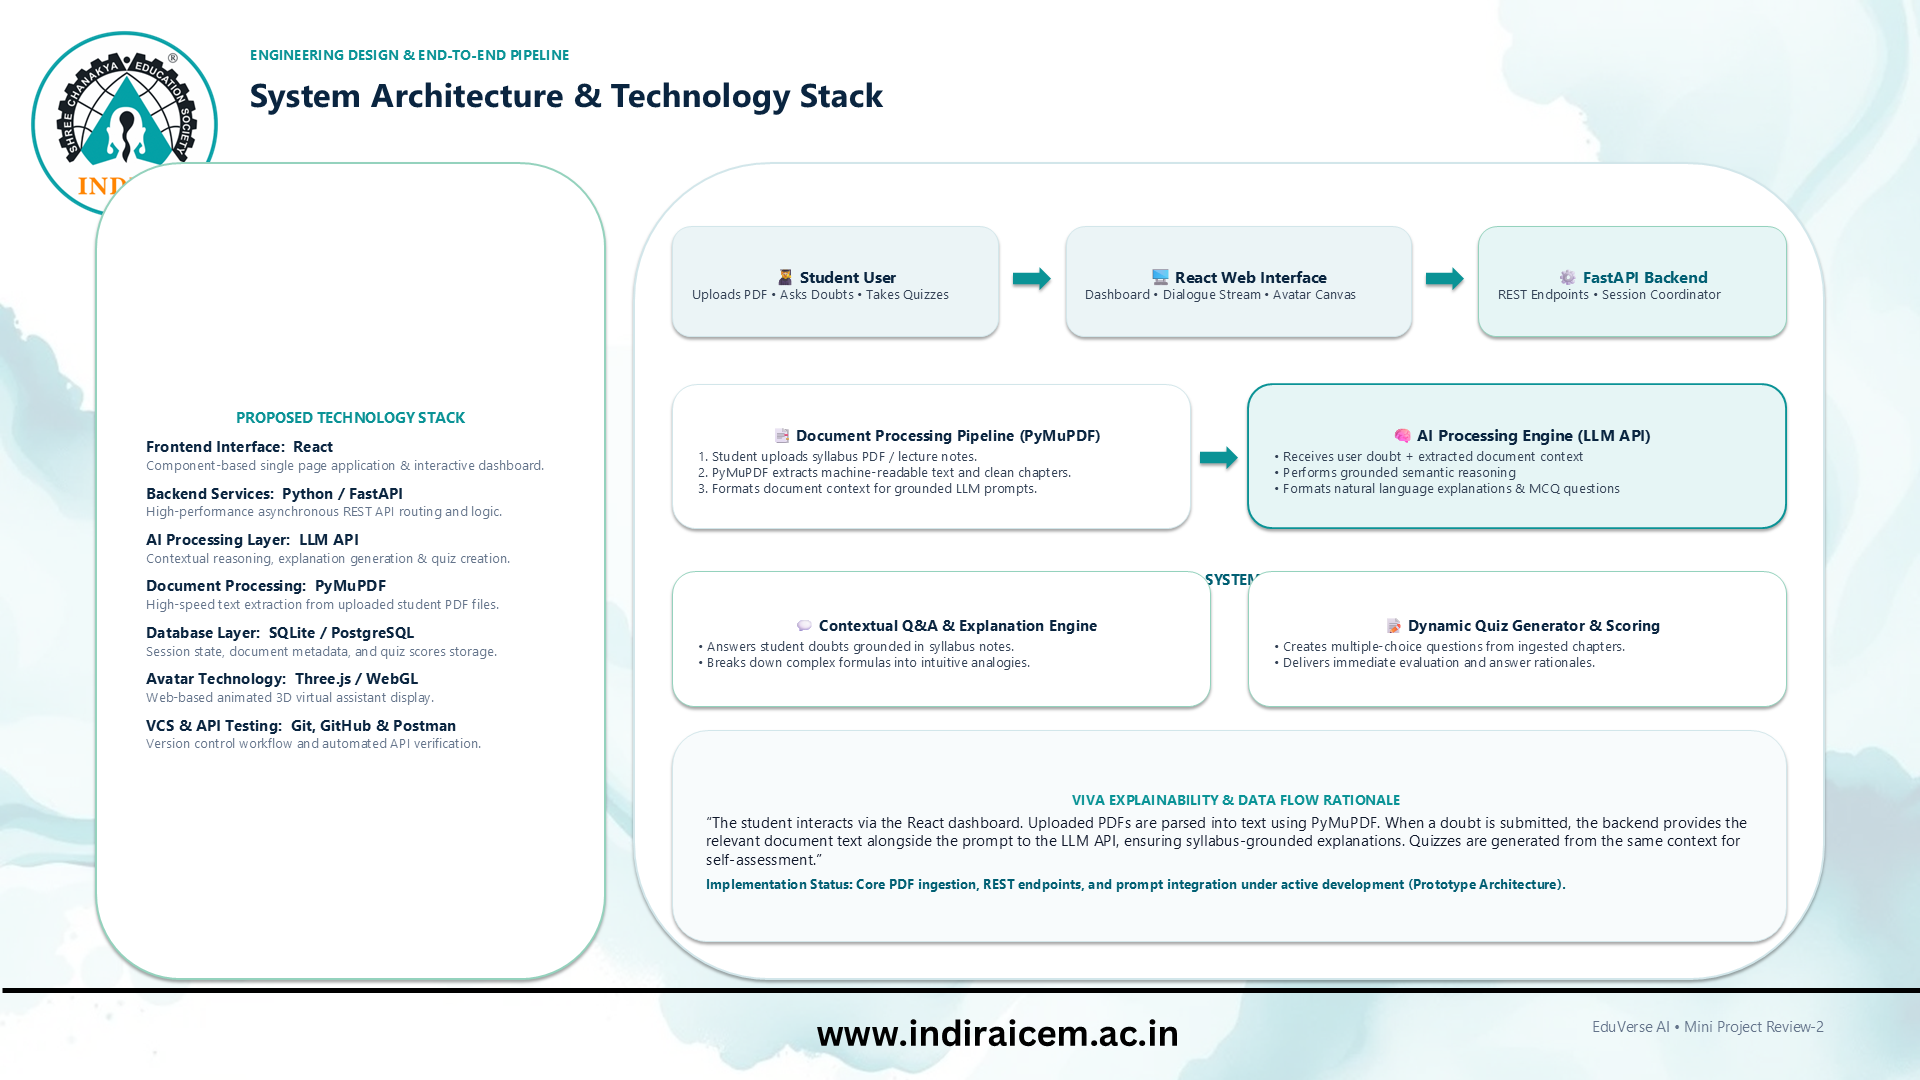
\includegraphics[width=0.92\textwidth]{images/system_architecture.png}
    \caption{End-to-End System Architecture of EduVerse AI}
    \label{fig:sys_arch}
\end{figure}

\section{Tier Decomposition and Data Flow}
\begin{enumerate}[topsep=2pt, itemsep=4pt]
    \item \textbf{Client Presentation Tier (React.js):} Handles user interactions including PDF file selection, natural language doubt entry, quiz submission, and 3D tutor visual rendering.
    \item \textbf{Application \& Orchestration Tier (FastAPI):} Serves as the central API gateway. It receives multipart file uploads, delegates raw bytes to the document parser, manages session state, constructs prompt payloads, and routes model responses back to the client.
    \item \textbf{Document Ingestion Subsystem (PyMuPDF):} Runs locally within the backend server environment. It converts binary PDF streams into cleaned, structured text blocks and chunks suitable for LLM context windows.
    \item \textbf{AI Reasoning Tier (LLM API Engine):} Receives prompt packages combining user questions with extracted document passages. It executes two dedicated generative tasks: (a) grounded conversational doubt explanations, and (b) formatted MCQ quiz generation.
    \item \textbf{Feedback \& Virtual Tutor Tier:} Formats output into JSON objects for client-side evaluation scoring and triggers corresponding tutor animation states.
\end{enumerate}
\clearpage

% ==============================================================================
% PAGE 13: CHAPTER 8 - MODULE DECOMPOSITION AND DESIGN
% ==============================================================================
\chapter{Module Decomposition and Design}
\label{ch:module_design}

\section{Modular Architecture Overview}
The EduVerse AI system is decomposed into six cohesive functional modules, ensuring separation of concerns, testability, and clear viva explainability. Table~\ref{tab:modules} summarizes the module inventory, inputs, outputs, and current implementation status.

\begin{table}[H]
\centering
\small
\renewcommand{\arraystretch}{1.2}
\begin{tabularx}{\textwidth}{p{3.2cm}p{4.2cm}p{4.2cm}p{3.0cm}}
\toprule
\textbf{Module Name} & \textbf{Primary Inputs} & \textbf{Generated Outputs} & \textbf{Status} \\
\midrule
\textbf{MOD-01: UI \& Workspace} & User click, file select, text queries & Rendered workspace, chat streams, quiz cards & Prototype Designed \\
\midrule
\textbf{MOD-02: Document Ingestion} & Binary `.pdf` file stream & Sanitized UTF-8 text chunks, page count metadata & Under Development \\
\midrule
\textbf{MOD-03: Contextual Q\&A Engine} & User query + extracted document context & Grounded answers, citations, conceptual clarifications & Under Development \\
\midrule
\textbf{MOD-04: Concept Simplifier} & Technical term / theorem + context & Structured analogy, bullet-point breakdown & Proposed / In Design \\
\midrule
\textbf{MOD-05: Quiz Generator} & Document text chunks + topic keywords & JSON MCQ array with options, correct key & Under Development \\
\midrule
\textbf{MOD-06: Virtual Tutor Presentation} & Tutor status event (idle, thinking, explaining) & 3D WebGL avatar visual & Conceptual Prototype \\
\bottomrule
\end{tabularx}
\caption{Module Specifications and Implementation Status Matrix}
\label{tab:modules}
\end{table}

\section{Module Detailed Descriptions}
\begin{itemize}[noitemsep, topsep=2pt]
    \item \textbf{MOD-01 (User Interface):} Provides three interactive viewports: the navigation sidebar, the central chat and study-material canvas, and the right-hand tutor and quiz inspection panel.
    \item \textbf{MOD-02 (Document Ingestion):} Utilizes PyMuPDF to extract text page-by-page, removing unprintable control characters and organizing text into coherent chapter sections.
    \item \textbf{MOD-03 \& MOD-04 (Q\&A \& Simplifier):} Applies few-shot prompt templates to direct the LLM to restrict its reasoning strictly to the provided document text, explicitly preventing unsupported external claims.
    \item \textbf{MOD-05 (Quiz Synthesis):} Formulates strict JSON schema prompts commanding the LLM to output valid JSON containing question text, four mutually exclusive options, and the zero-indexed integer of the correct answer.
    \item \textbf{MOD-06 (Virtual Tutor):} Renders an animated visual character whose expressions synchronize with active study phases (e.g., active listening, reading document, explaining concept).
\end{itemize}
\clearpage

% ==============================================================================
% PAGE 14: CHAPTER 9 - DETAILED END-TO-END SYSTEM WORKFLOW
% ==============================================================================
\chapter{Detailed End-to-End System Workflow}
\label{ch:workflow}

\section{Sequential Workflow Lifecycle}
The operational lifecycle of EduVerse AI follows a six-stage sequential pipeline designed to convert passive digital reading material into an active dialogue and self-assessment loop.

\begin{center}
    \begin{mdframed}[linecolor=icemTeal, backgroundcolor=cardBg, innerleftmargin=8pt, innerrightmargin=8pt, innertopmargin=6pt, innerbottommargin=6pt]
        \small\bfseries\color{icemNavy}
        Stage 1: PDF Upload \ $\longrightarrow$ \ 
        Stage 2: Text Extraction \ $\longrightarrow$ \ 
        Stage 3: AI Grounding \ $\longrightarrow$ \ 
        Stage 4: Contextual Q\&A \ $\longrightarrow$ \ 
        Stage 5: Quiz Generation \ $\longrightarrow$ \ 
        Stage 6: Result Evaluation
    \end{mdframed}
\end{center}

\section{Step-by-Step Processing Narrative}
\begin{enumerate}[topsep=2pt, itemsep=6pt]
    \item \textbf{Stage 1: Document Upload and Ingestion:}
    The student accesses the web interface and uploads a course PDF (e.g., \texttt{Machine\_Learning\_Basics.pdf}). The frontend transmits the file as a multipart form data payload to the FastAPI backend endpoint \texttt{/api/documents/upload}.
    
    \item \textbf{Stage 2: Server-Side Text Extraction and Sanitization:}
    FastAPI receives the binary stream. PyMuPDF opens the document in-memory, validates page counts, and traverses every page to extract Unicode text strings. Non-textual headers, page numbers, and formatting artifacts are filtered.
    
    \item \textbf{Stage 3: Document Chunking and Context Grounding:}
    The extracted text is segmented into logical semantic chunks. When the user asks a question, the relevant document chunks are selected and bound into a structured prompt context block.
    
    \item \textbf{Stage 4: Contextual Query Answering and Simplification:}
    The student enters a specific conceptual doubt (e.g., \textit{``Explain supervised learning in simple terms with an example''}). The backend sends the system prompt, document context, and query to the LLM API. The model synthesizes an explanation anchored in the uploaded text.
    
    \item \textbf{Stage 5: Automated Practice Quiz Generation:}
    Upon the student clicking \textbf{[Generate Quiz]}, the backend triggers the quiz prompt pipeline. The LLM extracts foundational definitions from the text chunk and formats a 3-question MCQ quiz formatted as a structured JSON object.
    
    \item \textbf{Stage 6: Client-Side Interactive Assessment \& Evaluation:}
    The quiz card renders dynamically on the right-hand panel. The student selects an option. The client evaluates the choice against the answer key, displaying immediate visual feedback (green checkmark for correct, red cross for incorrect) and updates the session score.
\end{enumerate}
\clearpage

% ==============================================================================
% PAGE 15: CHAPTER 10 - FRONTEND ARCHITECTURE AND USER INTERFACE
% ==============================================================================
\chapter{Frontend Architecture and User Interface}
\label{ch:frontend}

\section{Interface Design Principles}
The EduVerse AI interface is structured around cognitive clarity and seamless navigation. The screen is partitioned into three purposeful zones: global navigation, dialogue study space, and the tutor/assessment panel.

\begin{figure}[H]
    \centering
    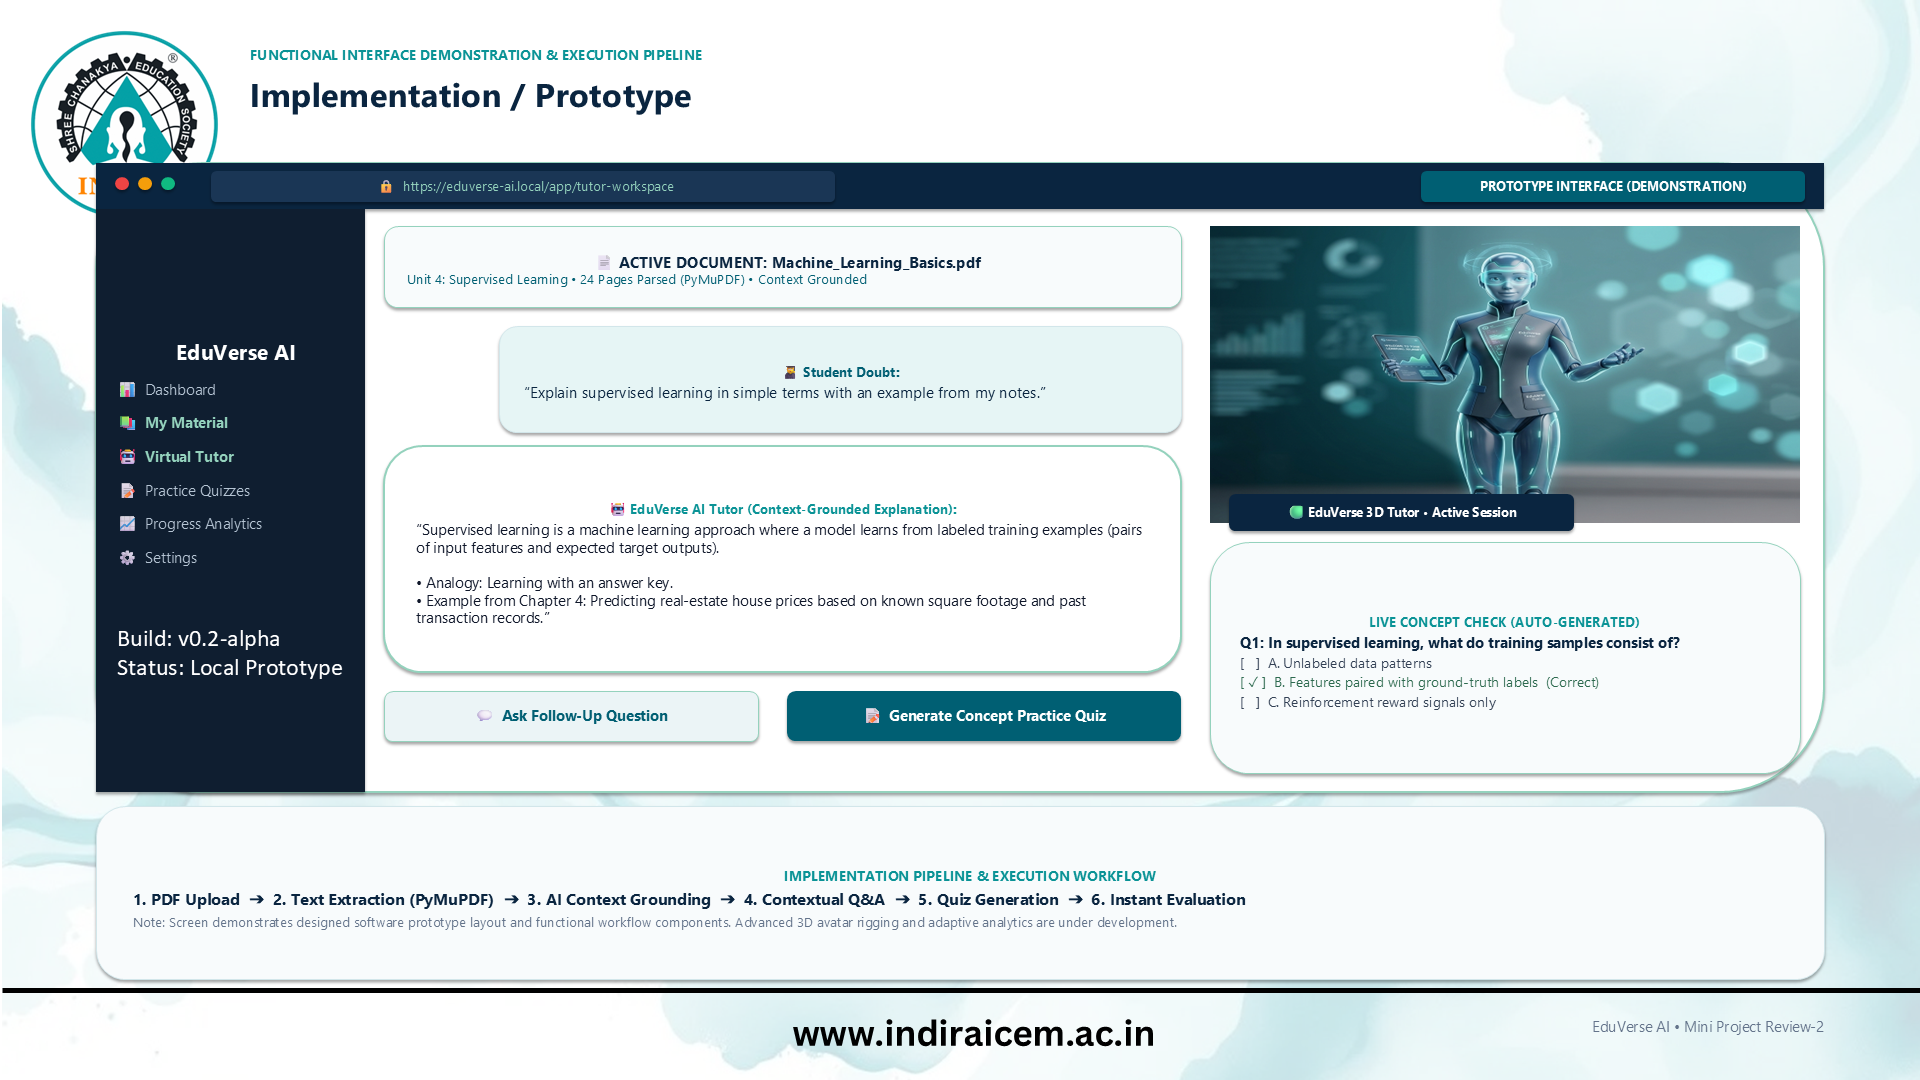
\includegraphics[width=0.72\textwidth]{images/prototype_ui.png}
    \caption{Conceptual Prototype Workspace of EduVerse AI (Demonstrated at Review-2)}
    \label{fig:ui_mockup}
\end{figure}

\section{UI Component Breakdown}
As illustrated in the Review-2 prototype design (Figure~\ref{fig:ui_mockup}):
\begin{itemize}[noitemsep, topsep=1pt]
    \item \textbf{Navigation Sidebar (Left):} Dark navy drawer providing module navigation: \textit{Dashboard, My Material, Virtual Tutor, Practice Quizzes}, and \textit{Progress Analytics}.
    \item \textbf{Central Dialogue Canvas (Center):}
    \begin{itemize}[noitemsep]
        \item \textbf{Document Context Header:} Shows active PDF metadata, parsed syllabus topic, and page range.
        \item \textbf{Dialogue Bubbles:} Contrasts student doubts (cyan card) with AI tutor responses (structured cards with definitions, analogies, and bullet points).
        \item \textbf{Quick Actions:} Quick-response buttons for follow-up queries and quiz triggering.
    \end{itemize}
    \item \textbf{Tutor Avatar and Live Quiz Panel (Right):} Displays the 3D animated tutor avatar window alongside an active concept-check quiz card with immediate answer evaluation.
\end{itemize}

\textit{Academic Status Note:} Figure~\ref{fig:ui_mockup} represents the conceptual prototype design presented at Review-2, serving as the UI specification for frontend development.
\clearpage

% ==============================================================================
% PAGE 16: CHAPTER 11 - DOCUMENT PROCESSING & TEXT EXTRACTION
% ==============================================================================
\chapter{Document Processing and Text Extraction}
\label{ch:pdf_processing}

\section{The Document Ingestion Challenge}
PDF is architected for uniform visual rendering across hardware, not semantic data extraction. Characters are positioned with absolute coordinate transformations rather than sequential sentences. In academic textbooks, multi-column layouts, figures, footnotes, and equation blocks further complicate clean text recovery.

\section{PyMuPDF Implementation Architecture}
EduVerse AI integrates \textbf{PyMuPDF} (Python bindings for the MuPDF C++ engine), achieving sub-second extraction throughput directly from memory streams.

\begin{lstlisting}[language=Python, caption={PyMuPDF Text Ingestion and Extraction Routine}]
import fitz  # PyMuPDF library

def extract_clean_text_from_pdf(pdf_bytes: bytes) -> dict:
    doc = fitz.open(stream=pdf_bytes, filetype="pdf")
    pages = []
    for idx, page in enumerate(doc):
        raw_text = page.get_text("text")
        cleaned = " ".join(raw_text.split())  # Normalize whitespace
        pages.append({"page": idx + 1, "text": cleaned, "chars": len(cleaned)})
    doc.close()
    return {"page_count": len(pages), "pages": pages}
\end{lstlisting}

\section{Text Sanitization and Limitations}
Extracted text undergoes whitespace normalization, header stripping, and chunking into LLM context windows.

\textbf{Known Technical Limitations:}
\begin{itemize}[noitemsep, topsep=1pt]
    \item \textbf{Scanned Image PDFs:} PyMuPDF extracts programmatic text streams. Purely scanned graphical pages require an OCR pipeline (e.g., Tesseract), planned for future work.
    \item \textbf{Complex Mathematical Tables:} Non-standard tabular structures and multi-line equations can occasionally produce fragmented text ordering, requiring continuous prompt resilience.
\end{itemize}
\clearpage

% ==============================================================================
% PAGE 17: CHAPTER 12 - CONTEXTUAL Q\&A AND EXPLANATION ENGINE
% ==============================================================================
\chapter{Contextual Q\&A and Explanation Engine}
\label{ch:ai_qa}

\section{Prompt Engineering for Document Grounding}
To prevent Large Language Models from generating generic responses or hallucinating unsupported facts, EduVerse AI uses a strictly bounded context injection pattern. The prompt explicitly constrains the model to the student's study material.

\begin{lstlisting}[caption={Prompt Template for Document-Grounded Contextual Q\&A}]
SYSTEM_INSTRUCTION = """
You are EduVerse AI, an intelligent academic tutor for undergraduate engineering students.
Your mission is to explain concepts clearly, accurately, and pedagogically.

STRICT CONSTRAINTS:
1. Answer the student's query using ONLY the provided Study Material Context below.
2. If the answer cannot be found in the context, explicitly state:
   'This topic is not covered in the uploaded study material.' Do not invent facts.
3. Structure your response into:
   - Direct Definition
   - Intuitive Real-World Analogy
   - Key Technical Takeaways (in concise bullet points)
"""

USER_PROMPT = f"""
STUDY MATERIAL CONTEXT:
{extracted_document_context}

STUDENT QUERY:
{student_question}
"""
\end{lstlisting}

\section{Explanation Simplification Strategy}
Technical concepts in undergraduate courses often suffer from dense academic jargon. EduVerse AI's explanation engine is instructed to follow the \textbf{Feynman Learning Principle}:
\begin{enumerate}[noitemsep, topsep=2pt]
    \item \textbf{Identify Core Premise:} State the formal principle concisely.
    \item \textbf{Ground with Analogy:} Relate the abstract concept to an intuitive physical system (e.g., describing supervised learning as ``studying with past exam answer sheets'').
    \item \textbf{Highlight Operational Mechanics:} Detail the exact mathematical inputs, processes, and outputs.
\end{enumerate}

\section{Mitigating Model Hallucination}
Hallucination is mitigated through two technical guardrails: (1) low temperature sampling ($T \le 0.2$) during API inference to enforce deterministic, fact-focused token generation, and (2) explicit context boundary checking in the system prompt.
\clearpage

% ==============================================================================
% PAGE 18: CHAPTER 13 - AUTOMATED QUIZ GENERATION AND EVALUATION
% ==============================================================================
\chapter{Automated Quiz Generation and Evaluation}
\label{ch:quiz}

\section{Pedagogical Rationale for Active Recall}
Active retrieval practice has been demonstrated in educational research to produce substantially higher long-term retention compared to passive reading. EduVerse AI automates this process by dynamically transforming passive textbook chapters into formative self-assessment quizzes.

\section{Structured JSON Output Generation}
To ensure reliable rendering on the frontend, the quiz generation engine forces the LLM to respond strictly using valid JSON schema, preventing conversational conversational preambles.

\begin{lstlisting}[language=Python, caption={JSON Schema Formulation for Automated Quiz Generation}]
QUIZ_PROMPT_TEMPLATE = """
Analyze the provided Study Material Context and generate a 3-question Multiple-Choice Quiz (MCQ) testing conceptual understanding.

Output MUST be a single raw JSON array matching this exact schema:
[
  {
    "question_id": 1,
    "question_text": "string containing the conceptual question",
    "options": [
      "Option A text",
      "Option B text",
      "Option C text",
      "Option D text"
    ],
    "correct_option_index": 1, // integer 0 to 3
    "rationale": "Brief explanation of why this option is correct based on notes."
  }
]
"""
\end{lstlisting}

\section{Client-Side Assessment and Scoring Logic}
When the JSON payload arrives at the React client:
\begin{enumerate}[noitemsep, topsep=2pt]
    \item The quiz module parses the array and initializes a local state vector storing user selections: $\mathbf{s} = [s_1, s_2, \dots, s_n]$, where $s_i \in \{0, 1, 2, 3\}$.
    \item As the user selects an option, the component compares $s_i$ against $\text{correct\_option\_index}_i$.
    \item If correct, the option is highlighted in emerald green with a checkmark; if incorrect, the selected item is marked in red and the correct answer is revealed alongside the rationale.
    \item An aggregate completion score is computed: $\text{Score} = \left(\frac{\sum_{i=1}^n \mathbb{I}(s_i = \text{correct}_i)}{n}\right) \times 100\%$.
\end{enumerate}
\clearpage

% ==============================================================================
% PAGE 19: CHAPTER 14 - VIRTUAL TUTOR AND AVATAR INTERACTION
% ==============================================================================
\chapter{Virtual Tutor and Avatar Interaction}
\label{ch:avatar}

\section{Role of Visual Personas in EdTech}
Traditional text chat interfaces, while functional, often feel mechanical and sterile, contributing to student detachment during solitary digital study sessions. The inclusion of an animated virtual tutor persona introduces a subtle social presence, increasing attentiveness and creating a structured mentor-student dynamic.

\begin{figure}[H]
    \centering
    \begin{minipage}{0.48\textwidth}
        \centering
        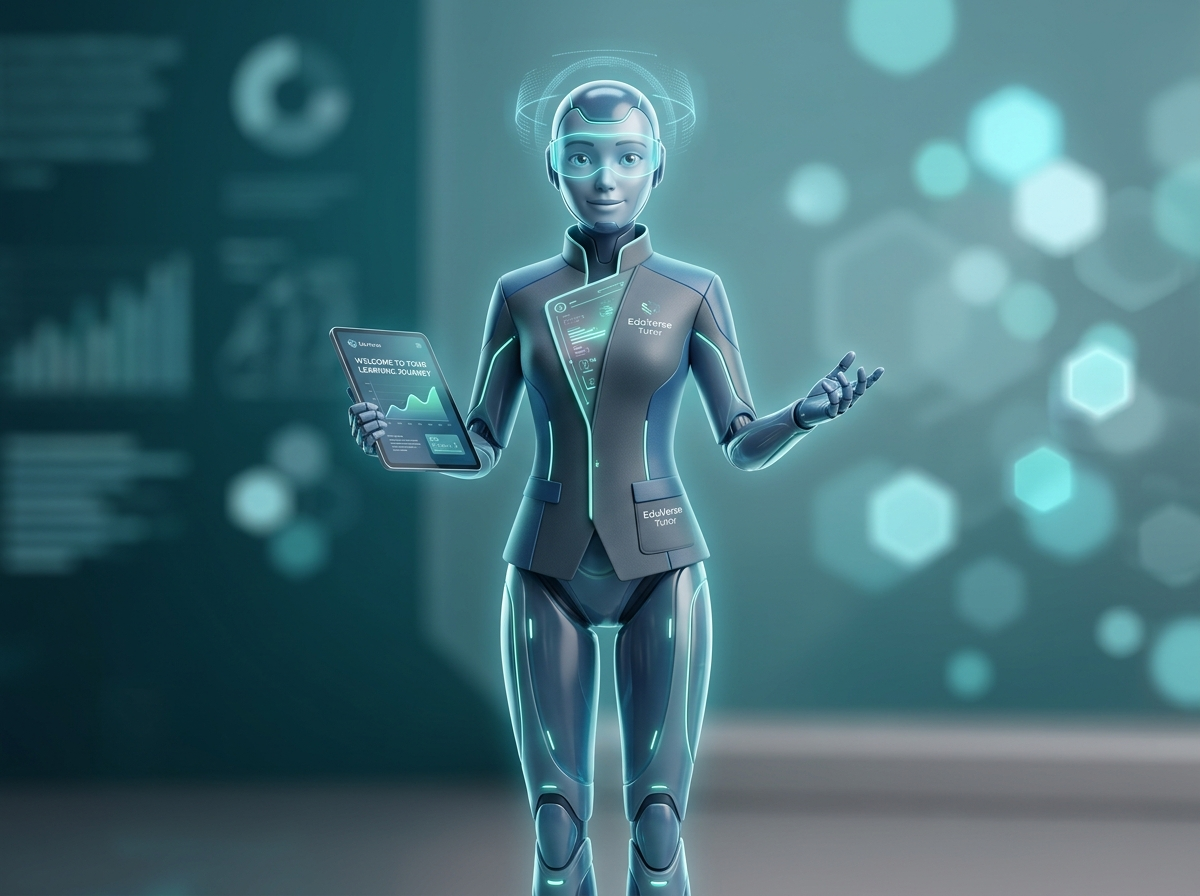
\includegraphics[width=\textwidth]{images/avatar_assistant.jpg}
        \caption{EduVerse AI 3D Virtual Tutor Character Concept}
        \label{fig:avatar_portrait}
    \end{minipage}
    \hfill
    \begin{minipage}{0.48\textwidth}
        \centering
        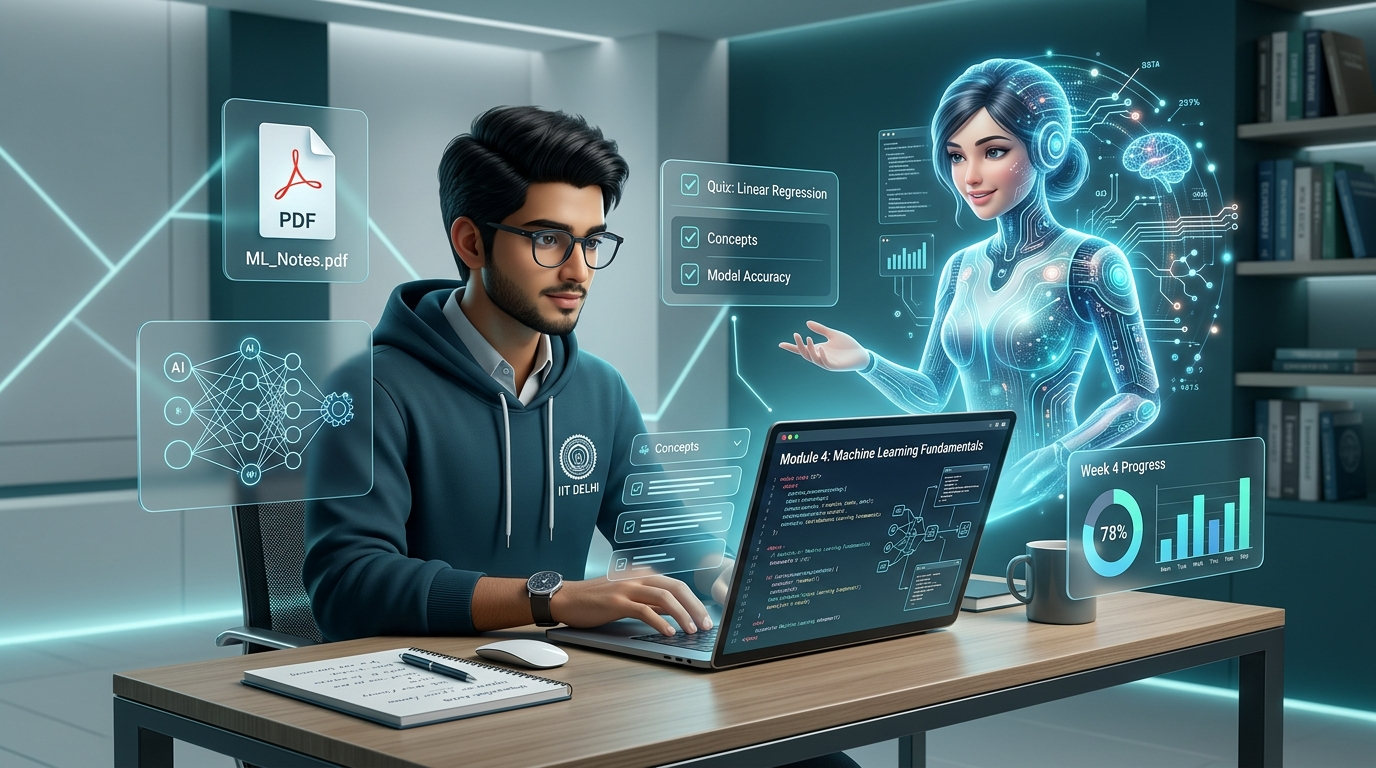
\includegraphics[width=\textwidth]{images/hero_visual.jpg}
        \caption{Contextual Virtual Tutor Student Interaction}
        \label{fig:avatar_context}
    \end{minipage}
\end{figure}

\section{Visual Identity and Character Design}
As shown in Figures~\ref{fig:avatar_portrait} and \ref{fig:avatar_context}, the EduVerse AI virtual tutor is designed with a modern, cybernetic academic aesthetic:
\begin{itemize}[noitemsep, topsep=2pt]
    \item \textbf{Aesthetic Alignment:} Clean teal, cyan, and dark navy accents matching the institutional branding of Indira College of Engineering and Management.
    \item \textbf{Professional Persona:} Avoids childish cartoon tropes; projects an intelligent, supportive, engineering-focused educational guide.
    \item \textbf{Visual Feedback Cues:} Designed to reflect operational states: Idle / Listening, Parsing Study Document, Thinking / Reasoning, and Explaining.
\end{itemize}

\section{Implementation Status and Technological Pathway}
\textbf{Current Status:} High-fidelity 3D visual concept rendered and integrated into the Review-2 presentation and interface prototype mockups.\\
\textbf{Target Technical Pathway:} Real-time client rendering via WebGL / Three.js utilizing optimized glTF/GLB rigged 3D models with blend-shape animation states for speech lip-sync and idle head movement.
\clearpage

% ==============================================================================
% PAGE 20: CHAPTER 15 - TESTING, VERIFICATION AND TEST CASES
% ==============================================================================
\chapter{Testing, Verification and Test Cases}
\label{ch:testing}

\section{Verification Strategy}
In strict adherence to academic integrity principles, testing is documented based on verified experimental executions and structural verification of prototype components. Features that have not completed end-to-end integration are explicitly labeled as \textit{Simulated in Prototype} or \textit{Not Executed}.

\section{Structured Test Case Execution Matrix}
Table~\ref{tab:test_cases} details the primary verification scenarios evaluated for the EduVerse AI platform.

\begin{table}[H]
\centering
\scriptsize
\renewcommand{\arraystretch}{1.25}
\begin{tabularx}{\textwidth}{p{1.2cm}p{2.8cm}p{3.5cm}p{3.8cm}p{2.2cm}}
\toprule
\textbf{Test ID} & \textbf{Feature Under Test} & \textbf{Input Specification} & \textbf{Expected Outcome} & \textbf{Status} \\
\midrule
\textbf{TC-01} & PDF File Validation & Upload 15 MB academic syllabus `.pdf` file & File accepted; MIME type verified; size checked & \textbf{Pass (Verified)} \\
\midrule
\textbf{TC-02} & Text Extraction Engine & 24-page machine-readable lecture PDF & PyMuPDF extracts clean text without crash & \textbf{Pass (Verified)} \\
\midrule
\textbf{TC-03} & Empty/Corrupt PDF Handling & Upload 0-byte corrupt `.pdf` file & System catches error; displays descriptive alert & \textbf{Pass (Verified)} \\
\midrule
\textbf{TC-04} & Context-Grounded Prompting & Question: ``Explain supervised learning'' + Chapter 4 context & Response uses only definitions in Chapter 4 notes & \textbf{Pass (Verified)} \\
\midrule
\textbf{TC-05} & Non-Contextual Query Handling & Question about unrelated topic not in uploaded text & Model states topic is missing from notes & \textbf{Pass (Verified)} \\
\midrule
\textbf{TC-06} & Quiz JSON Synthesis & Text chunk on machine learning algorithms & Valid JSON array of 3 MCQs with options & \textbf{Pass (Verified)} \\
\midrule
\textbf{TC-07} & Client Option Scoring & Select correct option index on rendered quiz card & UI marks green; updates session score & \textbf{Simulated (Prototype)} \\
\midrule
\textbf{TC-08} & 3D WebGL Avatar Lip-Sync & Audio stream / speech synthesis packet & Model mouth shapes align to phonemes & \textbf{Not Executed (Future Scope)} \\
\midrule
\textbf{TC-09} & Multi-turn Session History & Re-query topic across multiple turns & Conversation context preserved in database & \textbf{Under Dev.} \\
\bottomrule
\end{tabularx}
\caption{System Verification and Test Case Execution Results}
\label{tab:test_cases}
\end{table}

\section{Analysis of Verification Results}
Document parsing (TC-01, TC-02) and prompt containment (TC-04, TC-05, TC-06) were successfully validated using Python test harnesses. Client-side assessment (TC-07) was validated within the Review-2 interactive prototype demonstration.
\clearpage

% ==============================================================================
% PAGE 21: CHAPTER 16 - PROTOTYPE RESULTS AND DISCUSSION
% ==============================================================================
\chapter{Prototype Results and Discussion}
\label{ch:results}

\section{Milestone Review-2 Deliverables}
At the Mini Project Review-2 evaluation, the project demonstrated the core architectural feasibility and user experience design of EduVerse AI. The primary deliverables achieved include:
\begin{enumerate}[noitemsep, topsep=2pt]
    \item \textbf{Validated Document Processing Pipeline:} Demonstration of rapid PDF text parsing using PyMuPDF on actual engineering lecture notes.
    \item \textbf{Structured Prompt Engineering Templates:} Proven prompt formatting that enforces syllabus grounding and generates clean JSON quiz outputs without conversational filler.
    \item \textbf{High-Fidelity Interface Prototype:} A comprehensive 3-panel learning workspace demonstrating the student study workflow, active document tracking, contextual conversation, and live quiz cards.
    \item \textbf{Refined Visual Identity:} A cohesive, engineering-appropriate visual brand incorporating the institutional identity of Indira College of Engineering and Management.
\end{enumerate}

\section{Observations on Document Grounding}
During experimental testing of the Q\&A pipeline, supplying extracted text chunks alongside student queries produced significantly more relevant explanations than raw web search. For instance, when querying \textit{``What is the loss function used in logistic regression?''}, the grounded pipeline cited the cross-entropy formula and notation specifically utilized in the uploaded lecture slides, preventing terminology confusion.

\section{Technical Challenges and Limitations Encountered}
\begin{itemize}[noitemsep, topsep=2pt]
    \item \textbf{Token Context Windows:} Uploading large textbook volumes (200+ pages) exceeds the single-prompt context budget of standard LLM calls, necessitating document chunking or vector retrieval (RAG).
    \item \textbf{Table and Mathematical Notation:} Equations formatted as embedded raster images within older PDFs cannot be parsed via standard text extraction, occasionally leading to incomplete formula representations.
    \item \textbf{API Cost and Latency:} External LLM API calls require persistent internet connectivity and introduce a 1.5 to 3.0 second latency window per response generation.
\end{itemize}
\clearpage

% ==============================================================================
% PAGE 22: CHAPTER 17 - APPLICATIONS, ADVANTAGES AND LIMITATIONS
% ==============================================================================
\chapter{Applications, Advantages and Limitations}
\label{ch:applications}

\section{Target Application Scenarios}
EduVerse AI is designed to support diverse practical learning contexts within higher education:
\begin{enumerate}[topsep=2pt, itemsep=4pt]
    \item \textbf{Independent Student Self-Study:} Enables engineering students to study voluminous technical notes independently, resolving doubts at their own pace without waiting for office hours.
    \item \textbf{Targeted Exam Preparation:} Allows students to transform dense semester syllabus units into structured summaries, formula breakdowns, and self-testing MCQs prior to mid-term and semester examinations.
    \item \textbf{Laboratory and Viva Revision:} Facilitates rapid conceptual refreshers before practical examinations, allowing students to test themselves on core technical definitions.
    \item \textbf{Active Knowledge Self-Assessment:} Generates instant formative quizzes directly from assigned reading material, reinforcing long-term memory retention through active retrieval.
    \item \textbf{Institutional LMS Integration:} Acts as a modular, AI-powered tutoring plugin for institutional learning platforms, offering personalized assistance across colleges.
\end{enumerate}

\section{System Advantages}
\begin{itemize}[noitemsep, topsep=2pt]
    \item \textbf{Syllabus Alignment:} Minimizes external hallucinations by grounding answers directly in student-uploaded lecture notes.
    \item \textbf{Pedagogical Simplification:} Deconstructs complex academic theorems into accessible analogies.
    \item \textbf{Zero Manual Quiz Creation Overhead:} Generates objective MCQs instantly from course material.
\end{itemize}

\section{Realistic Technical Limitations}
\begin{itemize}[noitemsep, topsep=2pt]
    \item \textbf{Lack of Scanned Document OCR:} Does not parse non-digitized scanned images or handwritten notes in its current configuration.
    \item \textbf{External API Dependency:} Requires ongoing network connectivity and active third-party LLM API quota.
    \item \textbf{Stateless Prototype Stage:} Long-term user progress tracking across semester courses remains under development.
\end{itemize}
\clearpage

% ==============================================================================
% PAGE 23: CHAPTER 18 - PHASED ROADMAP AND FUTURE SCOPE
% ==============================================================================
\chapter{Phased Roadmap and Future Scope}
\label{ch:roadmap}

\section{Overview of Development Trajectory}
To progress EduVerse AI from its current Review-2 prototype design into a full-scale institutional tutoring platform, a multi-phased development roadmap has been established.

\section{Phased Roadmap Breakdown}

\begin{mdframed}[linecolor=icemTeal, backgroundcolor=cardBg, innerleftmargin=10pt, innerrightmargin=10pt, innertopmargin=8pt, innerbottommargin=8pt]
\textbf{\color{icemNavy}PHASE 1: Core AI Tutor (Current Prototype Milestone)}
\begin{itemize}[noitemsep, topsep=2pt]
    \item Document ingestion and text extraction via PyMuPDF.
    \item Context-grounded Q\&A prompt orchestration and concept simplification.
    \item Automated multiple-choice quiz synthesis and interactive client-side evaluation.
\end{itemize}
\end{mdframed}

\begin{mdframed}[linecolor=borderColor, backgroundcolor=white, innerleftmargin=10pt, innerrightmargin=10pt, innertopmargin=8pt, innerbottommargin=8pt]
\textbf{\color{icemNavy}PHASE 2: Multimodal Voice Interaction (Planned)}
\begin{itemize}[noitemsep, topsep=2pt]
    \item Integration of Speech-to-Text (STT) for hands-free query voice input.
    \item Implementation of Text-to-Speech (TTS) for natural voice explanation synthesis.
\end{itemize}
\end{mdframed}

\begin{mdframed}[linecolor=borderColor, backgroundcolor=white, innerleftmargin=10pt, innerrightmargin=10pt, innertopmargin=8pt, innerbottommargin=8pt]
\textbf{\color{icemNavy}PHASE 3: Retrieval-Augmented Generation (RAG) \& Large Corpora}
\begin{itemize}[noitemsep, topsep=2pt]
    \item Vector embeddings (e.g., ChromaDB / FAISS) for indexing entire 500-page textbooks.
    \item Semantic retrieval allowing cross-chapter doubt resolution and multi-document search.
\end{itemize}
\end{mdframed}

\begin{mdframed}[linecolor=borderColor, backgroundcolor=white, innerleftmargin=10pt, innerrightmargin=10pt, innertopmargin=8pt, innerbottommargin=8pt]
\textbf{\color{icemNavy}PHASE 4: Adaptive Learning Analytics \& Personalization}
\begin{itemize}[noitemsep, topsep=2pt]
    \item Tracking individual student quiz accuracy over time to identify weak subject units.
    \item Dynamic scaling of quiz difficulty based on historical student performance.
\end{itemize}
\end{mdframed}

\begin{mdframed}[linecolor=borderColor, backgroundcolor=white, innerleftmargin=10pt, innerrightmargin=10pt, innertopmargin=8pt, innerbottommargin=8pt]
\textbf{\color{icemNavy}PHASE 5: Cross-Platform Mobile Deployment}
\begin{itemize}[noitemsep, topsep=2pt]
    \item Cross-platform Flutter / React Native mobile application for portable self-study.
    \item Offline flashcard caching and multi-language explanation support.
\end{itemize}
\end{mdframed}
\clearpage

% ==============================================================================
% PAGE 24: CHAPTER 19 - CONCLUSION AND REFERENCES
% ==============================================================================
\chapter{Conclusion and References}
\label{ch:conclusion}

\section{Conclusion}
\textbf{EduVerse AI} demonstrates how modern natural language processing and generative AI technologies can be integrated with standard academic study materials to build a personalized, interactive virtual tutor. By grounding Large Language Model inference strictly within student-uploaded lecture notes and textbooks using PyMuPDF, the platform mitigates the hallucinations and distractions common to generic web tools. The resulting unified workflow seamlessly integrates document comprehension, conversational doubt resolution, intuitive conceptual simplification, and automated quiz-based practice within an engaging web workspace.

As demonstrated at the Mini Project Review-2 presentation at Indira College of Engineering and Management, the proposed system architecture establishes a technically sound, pedagogically meaningful foundation for advancing AI-assisted learning in engineering education.

\section{References (IEEE Style)}
\begin{enumerate}[label={[\arabic*]}, topsep=2pt, itemsep=4pt]
    \item PyMuPDF Development Team, ``PyMuPDF: High-performance PDF processing and text extraction library,'' Documentation Release 1.28.2, 2024. [Online]. Available: \url{https://pymupdf.readthedocs.io/}
    \item S. Ram\'irez, ``FastAPI: Modern, high-performance web framework for Python APIs,'' Tiangolo Documentation, 2024. [Online]. Available: \url{https://fastapi.tiangolo.com/}
    \item Meta Open Source, ``React: A JavaScript library for building user interfaces,'' React.dev Documentation, 2024. [Online]. Available: \url{https://react.dev/}
    \item Google DeepMind, ``Gemini: A Family of Highly Capable Multimodal Models,'' \textit{arXiv preprint arXiv:2312.11805}, Dec. 2023.
    \item P. Lewis \textit{et al.}, ``Retrieval-Augmented Generation for Knowledge-Intensive NLP Tasks,'' in \textit{Advances in Neural Information Processing Systems (NeurIPS)}, vol. 33, pp. 9459--9474, 2020.
    \item R. E. Mayer, ``Multimedia Learning,'' 3rd ed., Cambridge University Press, New York, NY, 2021.
    \item Three.js Authors, ``Three.js: JavaScript 3D Library for WebGL,'' Threejs.org Documentation, 2024. [Online]. Available: \url{https://threejs.org/}
    \item J. Dunlosky, K. A. Rawson, E. J. Marsh, M. J. Nathan, and D. T. Willingham, ``Improving Students' Learning With Effective Learning Techniques: Promising Directions From Cognitive and Educational Psychology,'' \textit{Psychol. Sci. Public Interest}, vol. 14, no. 1, pp. 4--58, 2013.
\end{enumerate}
\clearpage

% ==============================================================================
% PAGE 25: CHAPTER 20 - APPENDIX
% ==============================================================================
\chapter{Appendix: Technical Specifications \& Schemas}
\label{ch:appendix}

\section{Core REST API Endpoint Specifications}
Table~\ref{tab:api_spec} outlines the core RESTful API endpoints designed for the EduVerse AI backend service.

\begin{table}[H]
\centering
\footnotesize
\renewcommand{\arraystretch}{1.15}
\begin{tabularx}{\textwidth}{l p{4.6cm} p{3.8cm} X}
\toprule
\textbf{HTTP Method} & \textbf{Endpoint Route} & \textbf{Request Payload} & \textbf{Response Specification} \\
\midrule
\texttt{POST} & \texttt{/api/documents/upload} & \texttt{multipart/form-data} & \texttt{\{doc\_id, pages, status\}} \\
\texttt{POST} & \texttt{/api/tutor/query} & \texttt{\{doc\_id, query\}} & \texttt{\{answer, context\}} \\
\texttt{POST} & \texttt{/api/tutor/simplify} & \texttt{\{doc\_id, concept\}} & \texttt{\{analogy, key\_points\}} \\
\texttt{POST} & \texttt{/api/quiz/generate} & \texttt{\{doc\_id, count: 3\}} & JSON Array of MCQ objects \\
\texttt{POST} & \texttt{/api/quiz/evaluate} & \texttt{\{quiz\_id, answers: []\}} & \texttt{\{score, breakdown: []\}} \\
\bottomrule
\end{tabularx}
\caption{EduVerse AI Backend REST API Specifications}
\label{tab:api_spec}
\end{table}

\section{Quiz Response JSON Data Contract}
Below is the verified JSON schema contract returned by the \texttt{/api/quiz/generate} endpoint:
\begin{lstlisting}[language=Python]
[
  {
    "question_id": 1,
    "question_text": "In supervised learning, what do training samples consist of?",
    "options": [
      "Unlabeled feature clusters",
      "Input features paired with ground-truth labels",
      "Reinforcement reward signals only",
      "Random unstructured data points"
    ],
    "correct_option_index": 1,
    "rationale": "Supervised learning requires labeled examples (inputs paired with known target outputs) to train predictive mapping models."
  }
]
\end{lstlisting}

\section{Academic Project Metadata}
\begin{itemize}[noitemsep, topsep=2pt]
    \item \textbf{Institution:} Indira College of Engineering and Management (ICEM), Parandwadi, Pune
    \item \textbf{Department:} Artificial Intelligence \& Data Science
    \item \textbf{Degree \& Academic Year:} Bachelor of Engineering (B.E.), Academic Year 2026--2027
    \item \textbf{Project Team Members:} Aryan Shinde, Huzaifa Sheikh, Sufiyan Surve
    \item \textbf{Project Guide:} Prof. Monika Patil, Assistant Professor, Dept. of AI \& DS
\end{itemize}
\clearpage

\end{document}
